\section{Introduction}
There have been several recent proposals to extend existing data management systems with native Machine Learning support (e.g., MLBase \cite{kraska2013mlbase}, MADLIB\cite{hellerstein2012madlib}, TupleWare\cite{crotty2014tupleware}).
While these extensions can dramatically reduce programmer effort in developing learning-driven applications, pre-processing or ``cleaning" data is still a serious bottleneck \cite{kandel2012}. 
Data are susceptible to various forms of corruption, or \emph{dirtiness}, such as missing, incorrect, or inconsistent values.
Industrial surveys have established that dirty data are prevalent \cite{Gartner}, and there is a growing industry around cleaning data \cite{fortunearticle}.
Machine Learning is known to be sensitive to data quality \cite{xiaofeature}, and improper handling of dirty data can lead to unreliable and error-prone predictions.

Supervised Machine Learning relies on correlating features with labels, and systematically corrupted data can lead to confouding correlations.
Consider a music recommender system in which due to a software bug, all users from Europe have an incorrect age attribute defaulted to ``18-24".
A recommendation model trained on this data may spuriously ``learn" a correlation relationship between the ``18-24" age group and music liked by European users.
While there is an extensive literature on robust Machine Learning, this work largely focuses on resilience to atypical outliers (i.e., age ``150") and not spurious correlations.

Such problems can be ameliorated by a variety of data cleaning techniques (see Rahm and Do \cite{rahm2000data} for a survey).
Recently, several scalable data cleaning frameworks have been proposed including BigDansing\cite{khayyat2015bigdansing}, SampleClean\cite{sampleclean}, and Katara \cite{chu2015katara}. 
Unfortunately, even with recent research results, data cleaning can be time consuming and economically infeasible\cite{wang1999sample}.
Programming data transformations to fix all problems manifest in the data requires substantial developer effort \cite{kandel2012}.
When scripted transformations do not suffice, crowdsourcing is a popular alternative with success in missing value filling and entity resolution (\cite{gokhale2014corleone, park2014crowdfill, sampleclean,chu2015katara}.
However, crowdsourcing comes at the cost of additional latency and significant monetary expense.

Thus, for many corrupted datasets, the analyst can only practically clean $k \ll N$ records.
Strict budgets pose a significant challenge to Machine Learning.
Machine Learning applications can require a large amount of training data to learn correlations between possibly hundreds of features and labels.
A small sample of clean data may not be able to support a viable Machine Learning model.
Likewise, training on partially cleaned data, where cleaned data is mixed with dirty data, can lead to dramtically incorrect models (Figure \ref{update-arch1}).
This leads to the central question that we explore in this work, namely, when and how to apply data cleaning in a Machine Learning model training pipeline to avoid the severe dependence on sample size.

\begin{figure}[t]
\centering
 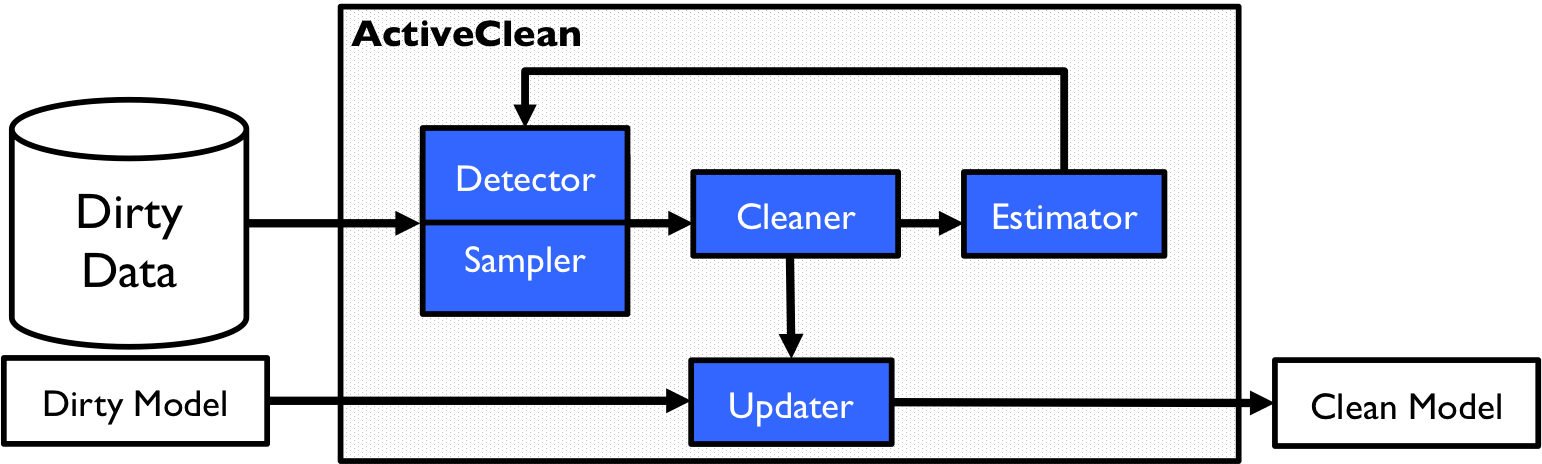
\includegraphics[width=\columnwidth]{figs/arch.png}
 \caption{\sysfull presents an architecture where data cleaning is integrated with model training. The user specifies a data cleaning procedure, and we provide a framework for sampling, model update, and feedback through estimation. \label{sys-arch}}\vspace{-2em}
\end{figure}

In this paper, we propose \sys, a framework that integrates existing data cleaning solutions with Machine Learning model training in a way that ensures reliable intermediate results.
Suppose an analyst has a large dirty dataset, a data cleaning technique, a budget of cleaning $k$ records, and a model she wishes to train.
\sys uses the model to select the most valuable samples of data to clean, and incrementally updates the model after cleaning.
The cleaning is iterative, applying the data cleaning procedure to samples and feeding the results back to adaptively select the next sample. 
\sys can integrate user specified dirty data detection rules (such as constraints) into the framework to further guide our sampling.
\sys supports a broad class of models, called convex-loss models, and a variety of data cleaning techniques (e.g., contraint-based, value filling, and entity resolution).
The key insight is that the iterative data cleaning and update process can be analyzed as a form of Stochastic Optimization \cite{bertsekas2011incremental} allowing us to leverage convex-analysis theory to develop optimized sampling and estimation methods.


As analytics frameworks increasingly support Machine Learning, tools that encourage appropriate methodologies are required.
The incremental updates from \sys give provable bounds on intermediate results and these results are also viable models that can be used for prediction. 
Specifically, our contributions are:
\begin{itemize}[noitemsep]
\item We propose a technique that updates a dirty model from clean data based on gradient descent.
\item We derive an optimal sampling distribution for estimating the gradient descent step, which while practically incomputable, can be approximated by maintaining an estimate of the impact of data cleaning on a record. 
\item The estimation technique applies linearization to decouple changes in different features allowing us to integrate knowledge about what is wrong with the data (i.e. analyst-specified detection rules) to better estimate error impact.
\item We show that batching together data that we expect to be clean can lead to significant improvements especially when the sample size is small.
\item We evaluate \sysfull on real and synthetic datasets to show that our approach gives a sharper cost-accuracy tradeoff than random sampling and Active Learning.
\end{itemize}






